\chapter{FET projects and social media}
This chapter presents an overview of the presence of FET projects on social media. Ut enim ad minim veniam, quis nostrum exercitationem ullam corporis suscipit laboriosam, nisi ut aliquid ex ea commodi consequatur. Quis aute iure reprehenderit in voluptate velit esse cillum dolore eu fugiat nulla pariatur. Excepteur sint obcaecat cupiditat non proident, sunt in culpa qui officia deserunt mollit anim id est laborum.

\section{Analysed FET projects} \label{Data_set}
This thesis focuses on the online communication activity of FET projects funded within Horizon 2020. The list of such projects was downloaded on 15th July 2017 from CORDIS, the main portal of the European Commission on results of EU-funded research projects. It consists of 151 projects and it is reported in Appendix \ref{List_of_FET_projects}. For each project, Appendix \ref{List_of_FET_projects} reports information on budget and start and end date, as well as the activated online communication channels. FET projects approved after 15th July 2017 are not considered in this thesis.  

Some of the projects in the list were not considered for this work. Excluded groups were the Flagship and Launchpad projects (see section \ref{The_FET_programme} for a brief description of the two groups), which were not considered representative of FET initiatives in terms of communication effort, as well as projects started after 1st February 2017. The lists of the excluded projects are reported in Appendix \ref{Specific_lists_of_FET_projects}. This procedure reduced the number of samples in the data set from 151 to 130.

Flagship projects were disregarded due to their budget.  As the available funding is far superior compared to the other FET projects, the Human Brain Project and the Graphene Flagships can invest larger resources on the communication activity. Thus, the two initiatives are outliers in the considered data set. 

Launchpad projects were not considered for this thesis as their ultimate goal is finding applications of results achieved by other FET projects and have limited interest in communication activity. Moreover, the available budget is relatively small. 

Finally, projects started after 1st February 2017 were disregarded as the time span between this date and the list download was judged insufficient to fully develop and launch an adequate communication activity. The only exception is the DEEP-EST project. In fact, by the time of writing DEEP-EST has already started its online communication activity.    

For some of the analyses in this thesis, the data set of 130 projects was divided into three sub-groups.  The first group consists of the 23 projects active in HPC and the transition to the exascale (see section \ref{FET_and_high-performing_computing}). The second subgroup includes the 12 projects in the field of quantum technologies (see section \ref{FET_and_quantum_technologies}). The third group comprises the other 95 projects. The lists of projects in the HPC and quantum technologies groups are reported in Appendix \ref{Specific_lists_of_FET_projects}. 

\section{Considered communication channels} \label{Considered_channels}
There exist disparate channels suitable for communication purposes. Those offering the widest audience are based on the internet. Examples are websites and social media. For this reason, FET projects consider the resources provided by the web as some of the main pillars of their communication strategy.

Different approaches can be considered to assess the use of online communication channels made by FET projects. One quantitative estimate is the fraction of projects active on specific platforms. For this thesis, the following communication channels were considered:   

\begin{description}
 \item [Website] The website is the online channel offering the highest degree of freedom to the owner. It allows the owner to personalise the content, the content's presentation strategy and the graphic visualisation.
 \item [Facebook] Facebook is the most used social media worldwide. It offers direct interaction among users and it is mainly designed for free time.  
 \item [Twitter] Twitter is very effective for concise science-related communication. It requires high posting rates and offers less personal interaction compared to Facebook.
 \item [Linkedin] Linkedin is ideal for professional content and enables the creation of closed groups. Nevertheless, interaction among users and outreach within the groups are limited.
 \item [YouTube] YouTube is the world's main platform for video sharing. It offers a very direct communication channel with effective monitoring tools. On the other hand, it is not very effective at engaging users and finding appropriate content may not be straightforward.
 \item [Instagram] Instagram has a very active and rapidly growing community. Effective communication via this channel requires pictures with strong visual content. Instagram offers limited interaction among users.
 \item [ResearchGate] ResearchGate offers the possibility to share technical documentation and engage in scientific discussions with researchers. As members are mainly scientists, the reachable community is significantly smaller and more homogeneous compared to other social networks.  
\end{description}

\section{Search for activated accounts}
The analyses presented in this thesis are based on the number of FET projects considering the online communication tools mentioned in section \ref{Considered_channels}. To this aim, a dedicated search was performed for all projects in Appendix \ref{List_of_FET_projects}. 

The search was conducted as follows. First, projects were contacted directly to ensure that the related information on the considered communication channels was complete. However, in some cases it was not possible to find the contact details of the project or no answer was received (dare numero). When this occurred, a desk search was performed to gather the required information. It cannot be excluded that the desk search failed to find the website or all accounts activated on the social channels considered for this thesis. Thus, it is highly probable that the list of accounts in Appendix \ref{List_of_FET_projects} is incomplete. The results presented in this thesis must therefore be considered as inferior limits when investigating the actual situation. 

\section{Overall presence} \label{Overall_presence}
Out of the 130 projects in the data set, ... have created a website, whereas ... have opened accounts on Twitter, ... on Facebook, ... on  Linkedin, ... on YouTube, ... on ResearchGate and ... on Instagram. The results, expressed in percentage, are shown in Figure \ref{Social_media}.

The results show that almost all FET projects have created a website. Facebook and Twitter are the two most popular social media within the FET community, hence reflecting the situation experienced in society. Nevertheless, the fraction of projects active on Twitter is significantly larger than that on Facebook. This is opposite to what occurs in society, where Facebook is the most used social media. This indicate that Twitter is considered a more suitable tool for scientific communication. 

\begin{figure}[!t] 
 \begin{center}
 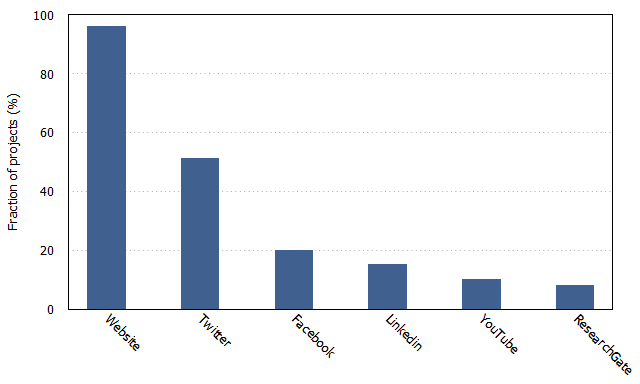
\includegraphics[scale=0.4]{Images/Social_media.png}
 \caption{Percentage of FET projects making use of the communication channels considered for this thesis.}
 \label{Social_media}
 \end{center}
\end{figure}

YouTube and Instagram are not common communication channels among FET projects. This is probably due to the difficulty of collecting visually impacting material capable of drawing attention of disparate audiences not familiar with the research field. The difficulty arises from the fact that the objectives and results of FET projects are often very technical and not appropriate for visual communication. In the case of YouTube, there is the additional problem of the high resources needed for the production of high-quality videos.

The number of projects active on ResearchGate is low. This is probably due to the fact that ResearchGate is not a suitable channel for large-scale communication activity. In fact, the reachable audience is typically limited to researchers active in similar investigation fields

\section{Presence breakdown}
The analysis in section \ref{Overall_presence} was repeated on the projects subgroups outlined in section \ref{Data_set}: HPC, QT and the others. This enable a comparison of how disparate classes of FET projects make use of online communication channels. The comparison among the three groups is shown in figure \ref{Social_media_breakdown}. 

The figure shows that websites are pillars of the communication strategies pursued by FET projects regardless of the subgroup. As for the most used social media within the FET community, i.e. Twitter, Facebook and Linkedin, the HPC subgroup has activated the most accounts compared to QT and other projects. The result indicates that HPC projects are among the most active FET initiatives in terms of online communication.  

QT projects seem to follow the opposite strategy. The number of projects making use of social media for their communication campaigns. is significantly smaller compared to HPC and other FET projects. In particular, none of them has activated an account on Twitter, the most used social platform in the FET community. 

The very limited use of social media made by QT projects highlights two facts. First, the online communication activity the QT Flagship will pursue will be designed without guidelines based on previous experiences from the same investigation field. Second, classes of projects facing similar challenges in terms of results communication and engagement of non-expert audiences may opt for very different strategies. This is the case of HPC and QT projects, as both pursue very technical goals which may look detached from society to the laymen. Moreover, the two classes target the common objective of improving current computers\footnote{Although HPC and QT projects focus on the development of present-day computers, the adopted strategies are very different: the former group aims at improving current classical architectures, the latter at exploiting a completely new approach, see sections \ref{FET_and_high-performing_computing} and \ref{FET_and_quantum_technologies}.}.

\begin{figure}[!t] 
 \begin{center}
 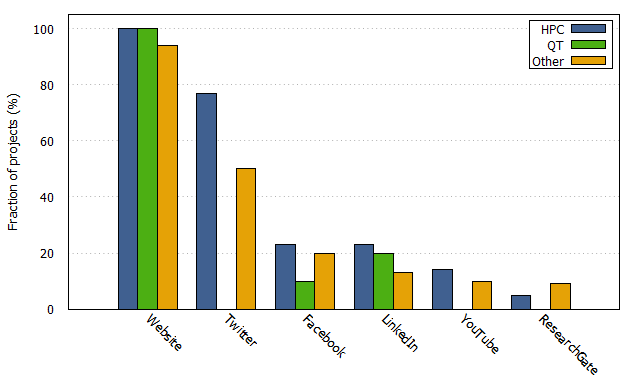
\includegraphics[scale=0.4]{Images/Social_media_breakdown.png}
 \caption{Percentage of FET projects making use of the communication channels considered for this thesis.}
 \label{Social_media_breakdown}
 \end{center}
\end{figure}

It must be beared in mind that the results presented in this section have been calculated on small data sets. The HPC and QT subgroups include ... and ... projects respectively, see Appendix \ref{Specific_lists_of_FET_projects}. The low number of projects indicates that results show limited robustness under even small changes in the data sets. The same applies to the percentages reported in figure \ref{Social_media_breakdown}. For example, the activation of a Twitter account from one single QT project would be sufficient to introduce significant variation of the result. Hence, the results reported in this section should rather serve as a guideline, and not as strong conclusions. 